\documentclass{article}
\usepackage[utf8]{inputenc}
\usepackage{tikz}
\usepackage{amssymb}
\usetikzlibrary{automata, positioning, arrows}
\newcommand{\blank}{\square}
\begin{document}
\begin{center}
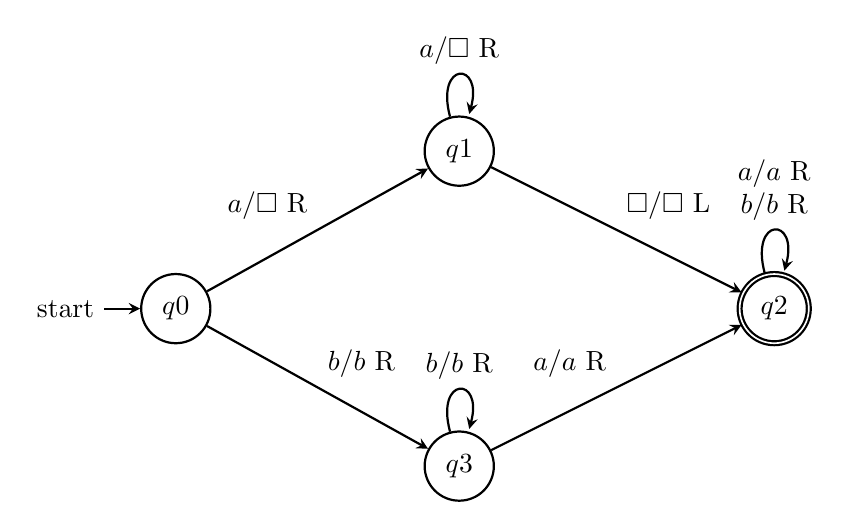
\begin{tikzpicture}[>=stealth, auto, node distance=2cm, thick]
    \node[state, initial] (0) at (2.00, -4.00) {$q0$};
    \node[state] (1) at (5.60, -2.00) {$q1$};
    \node[state, accepting] (2) at (9.60, -4.00) {$q2$};
    \node[state] (3) at (5.60, -6.00) {$q3$};

    \path[->]
        (0) edge[] node[align=center] {$a$/$\blank$ R} (1)
        (1) edge[loop above] node[align=center] {$a$/$\blank$ R} (1)
        (1) edge[] node[align=center] {$\blank$/$\blank$ L} (2)
        (0) edge[] node[align=center] {$b$/$b$ R} (3)
        (3) edge[loop above] node[align=center] {$b$/$b$ R} (3)
        (3) edge[] node[align=center] {$a$/$a$ R} (2)
        (2) edge[loop above] node[align=center] {$a$/$a$ R \\ $b$/$b$ R} (2)
    ;
\end{tikzpicture}
\end{center}
\end{document}